\documentclass[a4paper,10pt]{article}

%%%% PRATIQUE POUR LES ALINEAS CHIANTS
\usepackage{indentfirst}

%%%% POUR L'OPTION LABEL= %%%
\usepackage{enumitem}

\setlength{\parindent}{30pt}
\setlength{\parskip}{1ex}
\setlength{\textwidth}{15cm}
\setlength{\textheight}{24cm}
\setlength{\oddsidemargin}{0.2cm}
\setlength{\evensidemargin}{-.7cm}
\setlength{\topmargin}{-.5in}

\usepackage{graphicx}
\usepackage{titling}
\usepackage{listings}
\lstset{%
  basicstyle=\scriptsize\sffamily,%
  commentstyle=\footnotesize\ttfamily,%
  frameround=trBL,
  frame=single,
  breaklines=true,
  showstringspaces=false,
  numbers=left,
  numberstyle=\tiny,
  numbersep=10pt,
  keywordstyle=\bf
}
\newcommand{\subtitle}[1]{%
  \posttitle{%
    \par\end{center}
    \begin{center}\large#1\end{center}
    \vskip0.5em}%
}
\title{\textbf{Low level inputs/outputs}}
\subtitle{M1 MoSIG : Operating Systems}
\author{Poupin Pierre \and Rouby Thomas}
\date{18/11/2014}

\begin{document}
\maketitle

\section{Introduction}

Architecture of a typical device :

\begin{figure}[h!]
  \begin{center}
    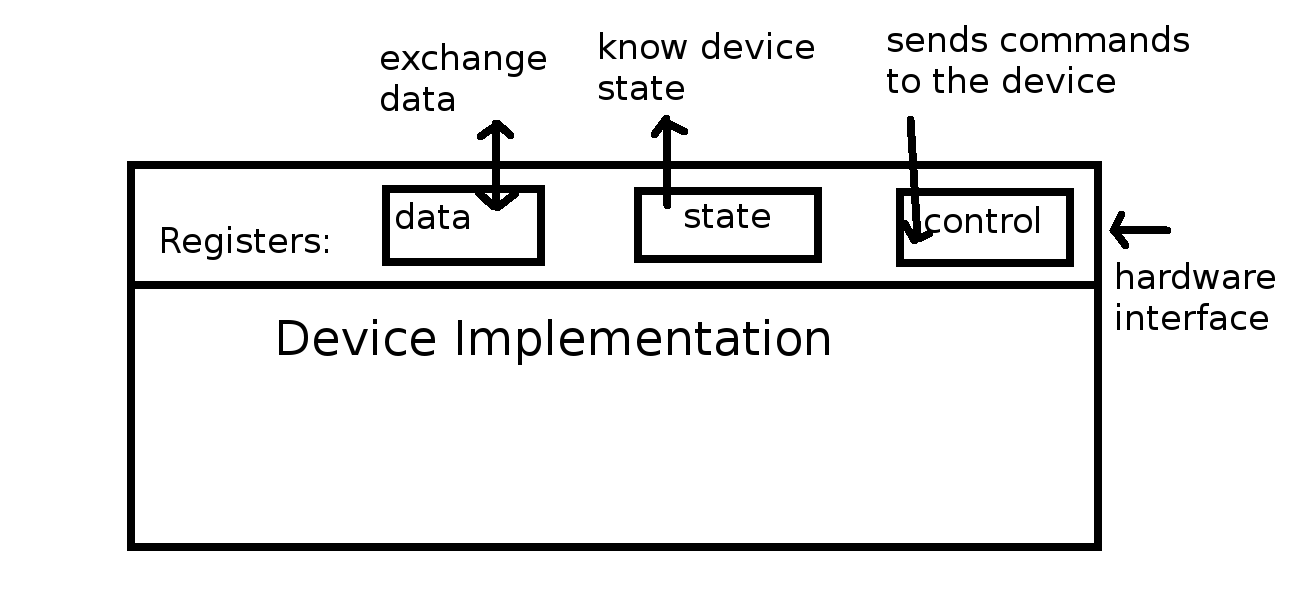
\includegraphics[width=0.8\textwidth]{architecture_device.png}
    \label{Architecture of a typical device}
  \end{center}
\end{figure}
This general scheme applies to : hard drives, printers, mouses...


Computer layout :
\begin{figure}[h!]
  \begin{center}
    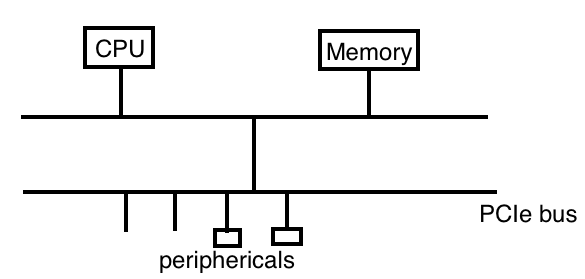
\includegraphics[width=0.8\textwidth]{computer_layout.png}
    \label{fig:}
  \end{center}
\end{figure}

To access to periphericals, one has to issue either :

\begin{itemize}
  \item special instructions to write to one of the I/O registers of periphericals.
  A port is provided which is the target device.
  
  \item memory access ... . The address space is divided into :
  \begin{itemize}
    \item  main memory
    \item 16 registers of periphericals
  \end{itemize}
\end{itemize}

Basic exchange with a peripherical :

\begin{verbatim}
  while(read(status) == busy) 
  {}
  write(data,some_data);
  write(control,some_command);
  while(read(status)==busy) 
  {}
\end{verbatim}



\section{Device Driver}

The OS would rather handle generic periphericals: for instance, a storage device should look like a sequence of data block

%place table here

Along with two properties :
\begin{itemize}
  \item 
\end{itemize}


\end{document}
